\chapter{SSB in Redis}
% TODO: Kapitel linken
Der \emph{Star Schema Benchmark} wurde ursprünglich für relationale Datenbanken entwickelt, die auf SQL basieren. Er ist nicht ohne weiteres auf Key-Value-Stores wie \emph{Redis} übertragbar. In diesem Kapitel wird erläutert, wie die Daten und Abfragen des SSB angepasst werden können, um den Benchmark in Redis durchführen zu können.

In Kapitel ~\ref{sec:ssb-data-in-redis} werden Ansätze vorgestellt, wie die Daten innerhalb von Redis strukturiert werden können. Im Anschluss daran wird das im Rahmen dieser Arbeit entwickelte Programm \emph{SSB Inserter} zum Einfügen der Daten in Redis vorgestellt.


Kapitel ~\ref{sec:ssb-use-in-redis} beschäftigt sich mit der Ausführung des SSB in Redis.
Zunächst wird das entwickelte Programm \emph{Redis OLAP Client} vorgestellt, welches zur Ausführung der Queries verwendet wurde. Anschließend werden verschiedene Ansätze zur Durchführung der Queries erläutert.

\section{Herausforderungen}
%\subsection{Keine Joins}

% TODO: Irgendwo noch Test von SSB in PostgreSQL
\section{SSB Daten in Redis}\label{sec:ssb-data-in-redis}

% TODO: Hier ganze Anleitung im Anhang verlinken
\subsection{Generieren von SSB Daten}
Um Daten für einen \emph{Star Schema Benchmark} zu generieren, stellen die Autoren ein spezielles Tool~\cite{phillips_electrumssb-dbgen_2023} zur Verfügung.
Das in \emph{C} programmierte Tool ermöglicht nach der Kompilierung die Erstellung von \emph{.tbl}-Dateien, welche für den Import in SQL-basierte Datenbanksysteme geeignet sind.
Es erlaubt die Variation der Datenmenge durch Anpassung eines Parameters, um unterschiedliche Skalierungen zu generieren.
Das Tool basiert auf einem Programm, das ursprünglich zur Datengenerierung für den TPC-H-Benchmark entwickelt wurde.
\begin{lstlisting}[
    caption=Auszug aus generierter supplier.tbl-Datei,
    label=code:ssb-dbgen-example,
    numbers=none
]
92|Supplier#000000092|n48Wy4QI3lm|BRAZIL   7|BRAZIL|AMERICA|12-446-416-8471|
93|Supplier#000000093|wd1djjKXT|MOZAMBIQU9|MOZAMBIQUE|AFRICA|26-359-388-5266|
\end{lstlisting}
Die Zeilen der .tbl-Datei repräsentieren eine Zeile in einer Datenbanktabelle. Die einzelnen Spalten sind durch einen Trennstrich voneinander getrennt.
Beim Importieren der Daten werden die Spalten den entsprechenden Spalten in der Datenbank zugeordnet. Dafür muss die Tabelle im korrekten Format erstellt werden.

\subsection{Sternschema in Redis abbilden}
Bei der Betrachtung der Datenorganisation gibt es grundlegende Unterschiede zwischen dem \emph{Sternschema} und den Möglichkeiten zur Datenmodellierung in \emph{Redis}. Während das Sternschema trotz einer geringeren Normalisierung als einige andere Schemata mehrere Tabellen umfasst, fehlt das Konzept der Tabelle in \emph{Redis} vollständig.

\subsubsection{Modellierung der Daten mit künstlichen Namensräumen}
Um dennoch eine Art Tabellenstruktur in \emph{Redis} zu erreichen, werden durch das Hinzufügen von Präfixen zu Schlüsseln künstliche Namensräume geschaffen. Alle Einträge, die der Tabelle \emph{Supplier} angehören, beginnen beispielsweise mit dem Präfix \enquote{supplier:}. Durch dieses Vorgehen ist es möglich, bei der Nutzung von Befehlen wie \emph{Scan} oder bei der Anwendung von Indizes in \emph{RediSearch} gezielt nach diesem Präfix zu suchen. Die Methode wird dabei von \emph{RedisInsight} unterstützt, das die Möglichkeit bietet, Daten in der Benutzeroberfläche nach Präfixen gruppiert anzuzeigen.

\begin{lstlisting}[
    caption=Beispiel von Keys mit künstlichem Namensräumen in Redis,
    label=code:redis-keys-example,
    numbers=none
]
supplier:1
lineorder:5:4
\end{lstlisting}


Es besteht die Möglichkeit, mehrere \emph{Datenbanken} in Redis anzulegen.
Dies wird jedoch als Anti-Pattern angesehen und ist daher nicht empfohlen~\cite{prickett_answer_2022}. Viele Erweiterungen unterstützen nur die erste Datenbank. Daher wird der Ansatz der künstlichen Namensräume bevorzugt. 

Neben der Option, die Struktur der \emph{SSB}-Daten durch künstliche Namensräume darzustellen, besteht auch die Möglichkeit, die Daten vollständig zu denormalisieren. Kapitel \ref{sec:ssb-inserter} beschreibt die Umsetzung beider Ansätze.


\subsubsection{Wahl des Datentypen in Redis}
Von den gängigen Datentypen in Redis unterstützen nur Hashes, JSON und Sorted Sets eine Key-Value-Struktur. Theoretisch können Daten auch in Strings gespeichert werden und durch die Volltextsuche von Redisearch ist es auch möglich nach Daten zu suchen, jedoch ist dies wesentlich komplizierter als bei Hashes und JSON.
In Sorted Sets können nur begrenzte numerische Werte gespeichert werden was sie für die SSB-Daten nicht nutzbar macht, da dort unter anderem auch Texte gespeichert werden müssen.
Hashes und JSON bieten beide die Möglichkeit, beliebige Daten in einer Key-Value-Struktur zu speichern und dann mir RediSearch auch nach diesen Daten zu suchen.
Hashes benötigen dafür jedoch erheblich weniger Speicherplatz als JSON.
JSON wird in einer deserialisierten Form gespeichert und benötigt etwas Overhead zusätzlich zu den eigentlichen Daten~\cite{redis_ltd_json-ram-usage_nodate}.
Hashes sind dagegen optimiert um Speicher zu sparen~\cite{redis_ltd_memory-optimization_nodate}.
Mit dem Befehl \lstinline|MEMORY USAGE| kann der Speicherverbrauch eines Elements in Redis angezeigt werden~\cite{redis_ltd_memory-usage-command-redis_nodate}.

% Dafür sorgen dass Abbildung an richitger Stelle ist...
In \Cref{pic:redis-hash-vs-json-memory} wird der Vergleich der Speicherplatznutzung dargestellt, wobei dieselben Informationen einmal in Form eines Hash und einmal in Form von JSON gespeichert sind. In diesem Beispiel belegt das JSON-Format 694 Byte, während das Hash-Format nur 288 Byte benötigt, was einer Reduzierung um 58,5\% entspricht.
\begin{figure}[!h]  % force the figure to be placed here
    \centering
    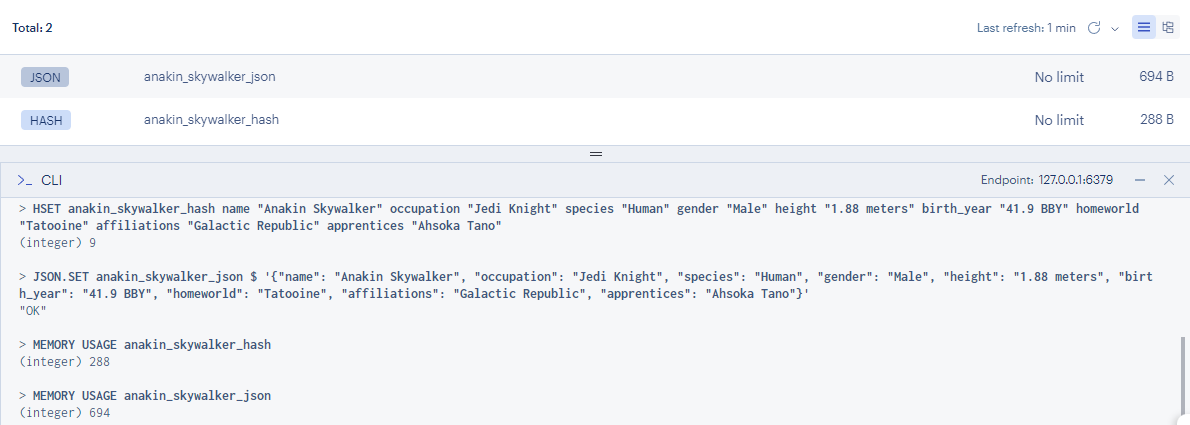
\includegraphics[width=1\textwidth]{pictures/redis/redis_hash_vs_json_memory.png}
    \caption{Vergleich der Speicherplatznutzung zwischen HASH und JSON}
    \label{pic:redis-hash-vs-json-memory}
\end{figure}

\subsection{SSB Inserter}\label{sec:ssb-inserter}

\subsubsection{Konfiguration von Redis und Jedis}
Redis verfügt über Eigenschaften, die beim Einfügen großer Datenmengen suboptimal sein können.
Es bietet die Möglichkeit, Daten sowohl als Snapshot als auch in einer Append-Only-Datei zu speichern (siehe Dokumentation von Redis~\cite{redis_ltd_persistence_nodate}).
Beim Einfügen von vielen Daten besteht die Gefahr, dass mehrfach Daten gespeichert werden, die in kurzer Zeit nicht mehr aktuell sind, wenn weitere Daten eingefügt werden. Aus diesem Grund wird beim Start des Programms sichergestellt, dass beide Optionen in der Konfiguration deaktiviert sind. Nachdem die Daten eingefügt wurden werden die Optionen wieder angepasst. 

Jedis hat außerdem einen Timeout für Anfragen. Um sicherzustellen, dass dieser Timeout das Einfügen der Daten nicht beendet, wird er auf unendlich gesetzt.

\begin{lstlisting}[
    caption=Optimierung beim Einfügen von Daten,
    label=code:ssb-inserter-redis-config,
    language=Java
]
// before inserting
jedis.configSet("appendonly", "no")
jedis.configSet("save", "")
jedis.getClient.setTimeoutInfinite()

// after inserting
jedis.configSet("appendonly", "yes")
jedis.configSet("save", "3600 1")
// perform snapshot every hour if at least one key has been changed
\end{lstlisting}


\subsubsection{Einfügen der Daten mit künstlichen Namensräumen}
% TODO: bissl drumrum ausbauen...
Um die Daten des \emph{SSB} in \emph{Redis} zu integrieren, ist es notwendig, zunächst die generierten \emph{.tbl}-Dateien zu lesen. Da in diesen Dateien keine Informationen zu den Spaltennamen enthalten sind, muss das Programm diese vergeben. Die benötigten Spaltennamen wurden aus dem SQL-Import-Skript entnommen, welches normalerweise zur Erstellung der Tabellen in \emph{PostgreSQL} verwendet wird.

Die Namen der Spalten sind in einem \emph{String}-Array innerhalb des \emph{Scala}-Programms gespeichert, wie in \Cref{code:ssb-inserter-datastructures} dargestellt:

\begin{lstlisting}[
    caption=Arrays mit den Namen der Spalten der SSB-Tabellen,
    label=code:ssb-inserter-datastructures,
    language=Java
]
val customerStructure: Array[String] =
  Array("c_custkey", "c_name", "c_address", "c_city", "c_nation", "c_region", "c_phone", "c_mktsegment")
val partStructure: Array[String] =
  Array("p_partkey", "p_name", "p_mfgr", "p_category", "p_brand1", "p_color", "p_type", "p_size", "p_container")
val dateStructure: Array[String] =
  Array("d_datekey", "d_date", "d_dayofweek", "d_month", "d_year", "d_yearmonthnum", "d_yearmonth", "d_daynuminweek", "d_daynuminmonth", "d_daynuminyear", "d_monthnuminyear", "d_weeknuminyear", "d_sellingseason", "d_lastdayinweekfl", "d_lastdayinmonthfl", "d_holidayfl", "d_weekdayfl")
val supplierStructure: Array[String] =
  Array("s_suppkey", "s_name", "s_address", "s_city", "s_nation", "s_region", "s_phone")
val lineorderStructure: Array[String] =
  Array("lo_orderkey", "lo_linenumber", "lo_custkey", "lo_partkey", "lo_suppkey", "lo_orderdate", "lo_orderpriority", "lo_shippriority", "lo_quantity", "lo_extendedprice", "lo_ordtotalprice", "lo_discount", "lo_revenue", "lo_supplycost", "lo_tax", "lo_commitdate", "lo_shipmod")

\end{lstlisting}


Der SSB Inserter liest zuerst jede \emph{.tbl}-Datei mit der Methode \lstinline|{readLines| ein. Dabei wird der Tabellenname aus dem Dateinamen extrahiert und die Datei in Zeilen gelesen. Die gelesenen Zeilen werden in Gruppen zu je 1000 Stück gebündelt. Für jede Gruppe wird die Funktion \lstinline|insertIntoRedis| aufgerufen, die die Daten in die Redis-Datenbank einfügt. Dabei wird der Tabellenname, ein Array mit den Spaltennamen, ein Jedis-Pipeline-Objekt und ein Boolean übergeben, der angibt, ob der Tabellenname \emph{lineorder} ist.
Zusätzlich wird die Zeit gemessen, die zum lesen und Einfügen der Daten benötigt wird.

\begin{lstlisting}[
    caption=Die Funktion readLines des SSB Inserter,
    label=code:ssb-inserter-readlines,
    language=Java
]
def readLines(fileName: String, dataStructure: Array[String], pipeline: Pipeline): Unit = {
	val tableName: String = fileName.split("\\.")(0);
	val startTime = System.nanoTime
	Try(Source.fromFile(fileName)) match {
		case Success(file) =>
			file.getLines().grouped(1000).foreach(s => insertIntoRedis(s, tableName, dataStructure, tableName == "lineorder", pipeline))
			println("Inserted data into " + tableName + " in " + (System.nanoTime() - startTime) + " nanoseconds")
			file.close()
		case Failure(exception) =>
			println("Could not read file `" + fileName + "`. It should be placed into the same folder as the .jar")
			println(exception.getMessage)
	}
}
\end{lstlisting}

Die Funktion \lstinline|insertIntoRedis| arbeitet wie folgt: Zunächst werden die vorliegenden Daten, die aus einer Folge von Zeilen bestehen, verarbeitet. Jede Zeile wird dabei anhand des Trennzeichen (\lstinline+|+) in einzelne Werte aufgeteilt. Anschließend wird für jedes Schlüsselelement im Array \emph{dataStructure} ein entsprechender Wert aus der aufgeteilten Zeile ausgewählt. Dann wird geprüft, ob die Option \emph{isLineOrder} aktiviert ist. Falls zutreffend, wird der Schlüssel für die Redis-Datenbank aus dem Namen der Datenbank und den ersten beiden Werten der Zeile gebildet. Andernfalls wird der Schlüssel lediglich aus dem Datenbanknamen und dem ersten Wert der Zeile erzeugt. Jedes Schlüssel-Wert-Paar wird dann in der Redis-Pipeline mit einem \emph{hset}-Befehl erzeugt, um den Wert unter dem jeweiligen Schlüssel in der Datenbank zu speichern.

\begin{lstlisting}[
    caption=Die Funktion insertIntoRedis des SSB Inserter,
    label=code:ssb-inserter-insertIntoRedis,
    language=Java
]
def insertIntoRedis(data: Seq[String], databaseName: String, dataStructure: Array[String], isLineOrder: Boolean, pipeline: Pipeline): Unit = {
	data.foreach(line => {
		val values = line.split("\\|")
		val valueIterator = values.iterator
		dataStructure.foreach(key => {
			if (valueIterator.hasNext) {
				if (isLineOrder) {
					pipeline.hset((databaseName + ":" + values(0) + ":" + values(1)).getBytes, key.getBytes, valueIterator.next().getBytes())
				} else {
					pipeline.hset((databaseName + ":" + values(0)).getBytes, key.getBytes, valueIterator.next().getBytes)
				}
			}
		})
	})
	pipeline.sync()
}
\end{lstlisting}

Um eindeutige Schlüsselnamen zu generieren, wird der Wert, der normalerweise als Primärschlüssel in relationalen Datenbanken verwendet wird, dem Tabellennamen angehängt. In der \emph{lineorder}-Tabelle ist dies ein zusammengesetzter Schlüssel, der aus zwei Feldern besteht. Aus diesem Grund ist es im Code notwendig, zwischen der \emph{lineorder}-Tabelle und den anderen Tabellen zu unterscheiden.

Die Daten werden gebündelt und in einer Pipeline an Redis übermittelt. Durch diese Bündelung auf maximal 1000 Elemente pro Pipeline wird die Häufigkeit der Kommunikation mit Redis reduziert. Das wiederum verbessert die Effizienz und Leistung, da weniger einzelne Anfragen nötig sind.


\subsubsection{Einfügen von denormalisierten Daten}
Beim denormalisierten Ansatz werden zuerst alle \emph{.tbl}-Dateien komplett geladen.

Für jede Tabelle gibt es eine passende Scala \emph{case class} die die notwendigen Daten für den SSB Benchmark enthalten. So gibt es die Klassen: \lstinline|ShortenedCustomerObject, ShortenedDateObject, ShortenedLineorderObject, ShortenedPartObject| und \lstinline|ShortenedSupplierObject|.

\begin{lstlisting}[
    caption=Das ShortenedCustomerObject,
    label=code:ssb-inserter-shortened-customer-object,
    language=Java
]
case class ShortenedCustomerObject(
	c_custkey: String,
	c_city: String,
	c_nation: String,
	c_region: String
								  )
\end{lstlisting}


Es ist zu berücksichtigen, dass ausschließlich die für die Queries notwendigen Felder enthalten sind. Die anderen Felder wurden entfernt, um Platz zu sparen und die Performance zu verbessern.

Für jede Tabelle wird eine Map definiert, die aus einem String als Key und der jeweiligen \emph{case class} als Value besteht.

Für jede Tabelle gibt es eine eigene Funktion, um die entsprechende Map zu füllen. Diese Funktionen folgen einem einheitlichen Schema: Sie verarbeiten die übergebenen Zeilen aus der gelesenen Datei, um eine Map zu erstellen, die anschließend einer der zuvor definierten Maps zugeordnet wird. Dabei besteht der Prozess darin, jede Zeile anhand des Trennzeichens \lstinline+|+ in ihre einzelnen Attribute zu gliedern. Aus diesen Attributen werden spezifische Objekte generiert, wobei nur die relevanten Teile der Zeilen verwendet werden. Dadurch entfallen sämtliche Werte, die nicht für die Abfrage benötigt werden. \cref{code:ssb-inserter-createCustomerMap} zeigt als Beispiel für eine solche Funktion die Funktion  \lstinline|createCustomerMap|, die genutzt wird, um die \emph{customer}-Map zu befüllen.

\begin{lstlisting}[
    caption=Die Funktion createCustomerMap,
    label=code:ssb-inserter-createCustomerMap,
    language=Java
]
def createCustomerMap(customerLines: Iterator[String]): Unit = {
	customerMap =
		customerLines.map(customerLine => {
			val attributes = customerLine.split('|')
			val customer = ShortenedCustomerObject(
				attributes(0),
				attributes(3),
				attributes(4),
				attributes(5)
			)
			(customer.c_custkey, customer)
		}).toMap
}
\end{lstlisting}


Die Funktion \lstinline|readLines| in Scala öffnet eine \emph{.tbl}-Datei, extrahiert den Namen der Tabelle aus dem Dateinamen und wendet die übergebene Funktion auf die Inhalte der Datei an. Die übergeben Funktion ist dabei die passende Funktion zur Erstellung einer Map zu dieser Tabelle, z.~B. \lstinline|createCustomerMap|. Nachdem die Datei geöffnet und die Zeilen an die Funktion übergeben wurden, wird die Datei geschlossen. Die Funktion integriert zusätzlich sowohl eine Zeitmessung zur Überwachung der Leistung als auch eine Fehlerbehandlung.

\begin{lstlisting}[
    caption=Die Funktion readLines für den denormalisierten Ansatz,
    label=code:ssb-inserter-readLines-denormalized,
    language=Java
]
def readLines(fileName: String, f: Iterator[String] => Unit): Unit = {
	val tableName: String = fileName.split("\\.")(0);
	val startTime = System.nanoTime
	Try(Source.fromFile(fileName)) match {
		case Success(file) =>
			f(file.getLines())
			file.close()
		case Failure(exception) =>
			println("Could not read file `" + fileName + "`. It should be placed into the same folder as the .jar")
			println(exception.getMessage)
	}
}
\end{lstlisting}

Um die Daten denormalisiert zu speichern, gibt es die \emph{case class} \lstinline|DenormalizedObject|. Sie enthält alle Felder, die für die Queries benötigt werden und kombiniert dabei die case classes der einzelnen Tabellen (siehe \cref{code:ssb-inserter-DenormalizedObject}).

\begin{lstlisting}[
    caption=Die case class DenormalizedObject,
    label=code:ssb-inserter-DenormalizedObject,
    language=Java
]
case class DenormalizedObject(
  lo_orderkey: String,
  lo_linenumber: String,
  lo_custkey: String,
  lo_discount: String,
  lo_extendedprice: String,
  lo_orderdate: String,
  lo_partkey: String,
  lo_quantity: String,
  lo_revenue: String,
  lo_suppkey: String,
  lo_supplycost: String,
  c_city: String,
  c_nation: String,
  p_category: String,
  s_city: String,
  s_nation: String,
  c_region: String,
  s_region: String,
  p_brand1: String,
  d_year: String,
  p_mfgr: String
							 )
\end{lstlisting}



Um eine Map mit denormalisierten Objekten zu erstellen, wird die Funktion \lstinline|createDenormalizedMap| genutzt. Diese verwendet die zuvor erstellten Maps der verschiedenen Tabellen. Die Funktion geht folgendermaßen vor: Zunächst wird jede Bestellung in \lstinline|lineorderMap| durchlaufen und für jeden Eintrag werden passende Objekte in den anderen Maps, also  \lstinline|customerMap|, \lstinline|supplierMap|, \lstinline|partMap| und \lstinline|dateMap|, gesucht. Dabei werden spezifische Schlüssel verwendet, die in den Bestellungen hinterlegt sind, z.~B. \lstinline|lo\_custkey|. In relationalen Datenbanken werden die Tabellen über diese Schlüssel verknüpft. Anschließend wird für jede Bestellung ein \lstinline|DenormalizedObject| erstellt, welches Informationen aus den entsprechenden Kundendaten, Lieferantendaten, Teildaten und Datumsobjekten mit den Bestelldaten kombiniert. Dieser Prozess führt zur Denormalisierung der Struktur, indem Daten aus verschiedenen Quellen zu einem einzigen Objekt zusammengeführt werden. Die denormalisierten Objekte werden dann in der \lstinline|denormalizedMap| gespeichert, wobei als Schlüssel der Key der \emph{lineorder}-Einträge verwendet wird.

\begin{lstlisting}[
    caption=Die Funktion createDenormalizedMap,
    label=code:ssb-inserter-createDenormalizedMap,
    language=Java
]
def createDenormalizedMap(

							 customerMap: Map[String, ShortenedCustomerObject],
							 supplierMap: Map[String, ShortenedSupplierObject],
							 partMap: Map[String, ShortenedPartObject],
							 lineorderMap: Map[String, ShortenedLineorderObject],
							 dateMap: Map[String, ShortenedDateObject]): Unit = {

	lineorderMap.foreach { case (key, lineorder) =>
		val customer = customerMap.getOrElse(lineorder.lo_custkey, ShortenedCustomerObject("", "", "", ""))
		val supplier = supplierMap.getOrElse(lineorder.lo_suppkey, ShortenedSupplierObject("", "", "", ""))
		val part = partMap.getOrElse(lineorder.lo_partkey, ShortenedPartObject("", "", "", ""))
		val date = dateMap.getOrElse(lineorder.lo_orderdate, ShortenedDateObject("", ""))

		val denormalized = DenormalizedObject(
			lineorder.lo_orderkey,
			lineorder.lo_linenumber,
			lineorder.lo_custkey,
			lineorder.lo_discount,
			lineorder.lo_extendedprice,
			lineorder.lo_orderdate,
			lineorder.lo_partkey,
			lineorder.lo_quantity,
			lineorder.lo_revenue,
			lineorder.lo_suppkey,
			lineorder.lo_supplycost,
			customer.c_city,
			customer.c_nation,
			part.p_category,
			supplier.s_city,
			supplier.s_nation,
			customer.c_region,
			supplier.s_region,
			part.p_brand1,
			date.d_year,
			part.p_mfgr
		)

		denormalizedMap += (key -> denormalized)
	}


}
\end{lstlisting}


Zum Schluss werden die Daten mit der Funktion \lstinline|insertDenormalizedObjectsIntoRedis| an Redis gesendet.
Die Funktion gruppiert die denormalisierten Objekte der \lstinline|denormalizedMap| in Gruppen zu je 1000, um die Einfügeeffizienz in Redis zu optimieren. Für jedes denormalisierte Objekt wird eine Map erstellt, die aus den Bezeichnungen der Attribute der Objekte als Schlüssel und den Attributen als Wert besteht. Anschließend werden diese Maps mittels einer Redis-Pipeline in die Datenbank übertragen, wobei sie als Hash in der Datenbank gespeichert werden. Für die Schlüssel der Hashes wird eine Kombination aus \lstinline|lo\_oderderkey| und \lstinline|lo\_linenumber| verwendet. Um die Transaktionen abzuschließen, wird die Pipeline nach dem Einfügen jeder Gruppe von 1000 Objekten synchronisiert.

\begin{lstlisting}[
    caption=Die Funktion insertDenormalizedObjectsIntoRedis,
    label=code:ssb-inserter-insertDenormalizedObjectsIntoRedis,
    language=Java
]
private def insertDenormalizedObjectsIntoRedis(pipeline: Pipeline): Unit = {
	denormalizedMap.values.grouped(1000).foreach(denormalizedObjects => {
		denormalizedObjects.foreach(denormalizedObject => {
			val hash = Map(
				"lo_orderkey" -> denormalizedObject.lo_orderkey,
				"lo_linenumber" -> denormalizedObject.lo_linenumber,
				"lo_custkey" -> denormalizedObject.lo_custkey,
				"lo_discount" -> denormalizedObject.lo_discount,
				"lo_extendedprice" -> denormalizedObject.lo_extendedprice,
				"lo_orderdate" -> denormalizedObject.lo_orderdate,
				"lo_partkey" -> denormalizedObject.lo_partkey,
				"lo_quantity" -> denormalizedObject.lo_quantity,
				"lo_revenue" -> denormalizedObject.lo_revenue,
				"lo_suppkey" -> denormalizedObject.lo_suppkey,
				"lo_supplycost" -> denormalizedObject.lo_supplycost,
				"c_city" -> denormalizedObject.c_city,
				"c_nation" -> denormalizedObject.c_nation,
				"p_category" -> denormalizedObject.p_category,
				"s_city" -> denormalizedObject.s_city,
				"s_nation" -> denormalizedObject.s_nation,
				"c_region" -> denormalizedObject.c_region,
				"s_region" -> denormalizedObject.s_region,
				"p_brand1" -> denormalizedObject.p_brand1,
				"d_year" -> denormalizedObject.d_year,
				"p_mfgr" -> denormalizedObject.p_mfgr
			)
			pipeline.hmset("lineorder:" + denormalizedObject.lo_orderkey + ":" + denormalizedObject.lo_linenumber, hash.asJava)
			numOfInsertedRecords = numOfInsertedRecords + 1
		})
		pipeline.sync()
	})
}
\end{lstlisting}




\section{SSB in Redis ausführen}\label{sec:ssb-use-in-redis}

\subsection{Redis OLAP Client}

\subsubsection{Konfiguration von RediSearch und Jedis}
Standardmäßig begrenzt RediSearch sowohl die Anzahl der Suchergebnisse als auch die der Aggregationsergebnisse (siehe Dokumentation von RediSearch~\cite{redis_ltd_configuration_nodate}). Außerdem verfügt RediSearch über einen Timeout für Abfragen. Um sicherzustellen, dass diese Begrenzungen bei der Verarbeitung großer Datenmengen nicht wirksam werden, werden sie deaktiviert.

Gleiches gilt für den Timeout von Jedis auf der Clientseite.
\begin{lstlisting}[
    caption=Konfiguration von RediSearch,
    label=code:redis-olap-client-config,
    language=Java
]
jedisPooled.sendCommand(SearchCommand.CONFIG, "SET", "MAXSEARCHRESULTS", "-1")
jedisPooled.sendCommand(SearchCommand.CONFIG, "SET", "MAXAGGREGATERESULTS", "-1")
jedisPooled.sendCommand(SearchCommand.CONFIG, "SET", "TIMEOUT", "0")

jedis.getClient.setTimeoutInfinite()
\end{lstlisting}

\section{4 Ansätze}
% TODO: Einleitungstext
\subsection{Ansatz 1: Alles in Keys}
\subsubsection{Aufbau der Daten}
\subsubsection{Aufbau der Abfragen}
\subsubsection{Ergebnisse}
\subsubsection{Fazit}


\subsection{Ansatz 2: Clientseitige Joins}

\subsubsection{Aufbau der Daten}\label{sec:client-approach-datastructure}
Dieser Ansatz beruht auf einer Struktur, in der die Daten so nah wie möglich an der ursprünglichen Datenstruktur gehalten werden, was durch die Verwendung künstlicher Namensräume erreicht wird. Konkret bedeutet dies, dass jede Zeile aller \emph{.tbl}-Dateien mit einem spezifischen Präfix in die Datenbank eingefügt wurde. . Für jeden dieser Namensräume wurde ein dedizierter Index erstellt. Bei der Erstellung dieser Indizes wurden nur die notwendigen Felder für den jeweiligen Kontext berücksichtigt.

Für den Namensraum der \emph{supplier}-Daten wurde ein Index erstellt, der ausschließlich das Feld \emph{s\_region} enthält. Dieses Feld wird als \emph{TAG} indiziert, da es Daten wie beispielsweise \lstinline|AMERICA| enthält.

\begin{lstlisting}[
    caption=Befehl zum Anlegen des Index für supplier-Daten,
    label=code:redis-index-supplier,
    numbers=none
]
FT.CREATE supplier-index PREFIX 1 "supplier:" SCHEMA s_region TAG
\end{lstlisting}


Ähnlich verhält es sich mit dem Index für die \emph{part}-Daten, der lediglich das Feld \emph{p\_category} umfasst. Dieses Feld wird als \emph{Tag} indiziert, da es Werte wie beispielsweise \lstinline|MFGR#54| enthält.

\begin{lstlisting}[
    caption=Befehl zum Anlegen des Index für part-Daten,
    label=code:redis-index-part,
    numbers=none
]
FT.CREATE part-index PREFIX 1 "part:" SCHEMA p_category TAG
\end{lstlisting}


Im Gegensatz dazu umfasst der Index für die \emph{Date}-Daten mehrere numerische Werte, nämlich \emph{d\_year}, \emph{d\_datekey}, \emph{d\_yearmonthnum} und \emph{d\_weeknuminyear}. 

\begin{lstlisting}[
    caption=Befehl zum Anlegen des Index für date-Daten,
    label=code:redis-index-date,
    numbers=none
]
FT.CREATE date-index PREFIX 1 "date:" SCHEMA d_year NUMERIC d_datekey NUMERIC d_yearmonthnum NUMERIC d_weeknuminyear NUMERIC
\end{lstlisting}


Schließlich enthält der Index für die \emph{Lineorder}-Daten eine Reihe von numerischen Werten, die für die Abwicklung und Analyse von Bestellungen relevant sind. Dies umfasst \emph{lo\_orderdate}, \emph{lo\_discount}, \emph{lo\_quantity}, \emph{lo\_partkey}, \emph{lo\_suppkey} und \emph{lo\_extendedprice}. Die Felder, die mit \enquote{key} enden, enthalten IDs der Werte aus den anderen Tabellen. Zum Beispiel steht \lstinline|lo_partkey=1389| für den Eintrag \lstinline|part:1389|.

\begin{lstlisting}[
    caption=Befehl zum Anlegen des Index für lineorder-Daten,
    label=code:redis-index-lineorder,
    numbers=none
]
FT.CREATE lineorder-index PREFIX 1 "lineorder:" SCHEMA lo_orderdate NUMERIC lo_discount NUMERIC lo_quantity NUMERIC lo_partkey NUMERIC lo_suppkey NUMERIC lo_extendedprice NUMERIC
\end{lstlisting}

\subsubsection{Aufbau der Abfragen}

Für die erste Query (Q1.1) werden im Original die Daten aus der Tabelle \emph{date} und der Tabelle \emph{lineorder} gejoint. Da Redis keine Möglichkeiten zum Joinen bietet, müssen die Daten clientseitig gejoint werden.

\begin{lstlisting}[
    caption=Originale SQL Query Q1.1 des SSB,
    label=code:ssb-q-1-1,
    language=Sql
]
select sum(lo_extendedprice*lo_discount) as revenue
  from lineorder, date
  where lo_orderdate = d_datekey
  and d_year = 1993
  and lo_discount between 1 and 3
  and lo_quantity < 25;
\end{lstlisting}

Dazu werden zuerst die relevanten \emph{date}-Datensätze geladen, da diese weniger Daten enthalten als die benötigten \emph{lineorder}-Datensätze. Im ersten Schritt werden also alle Einträge aus dem \emph{date-index} abgefragt, bei denen \lstinline|d_year=1993|. Bei der Abfrage wird angegeben, dass nur das Feld \lstinline|d_datekey| zurückgegeben werden soll.

\begin{lstlisting}[
    caption=Abfragen der date-Daten für Q1.1 im Redis Olap Client,
    label=code:redis-olap-server-q1-1-date,
    language=Java
]
val dateFilters: List[Query.Filter] = List(new Query.NumericFilter("d_year", 1993, 1993))
val dateDocuments: List[Document] = queryDocuments(jedisPooled, "date-index", filters = dateFilters, List("d_datekey"))
\end{lstlisting}

Im Anschluss wird ein Query-String für die \emph{lineorder}-Daten erzeugt, indem für jedes Dokument, das aus dem \emph{date-index} abgerufen wird, eine Datumsbereichsabfrage erstellt wird. Diese Abfragen werden in einer Liste zusammengefasst und mit dem Trennzeichen \enquote{|} (logisches Oder) zu einem einzigen RediSearch-Abfragestring kombiniert. Dieser Ansatz ermöglicht die Kombination mehrerer spezifischer Datumsabfragen in einer einzigen Datenbankabfrage.

\begin{lstlisting}[
    caption=Erstellen eines Query-Strings mit Datumsbereichen für Q1.1,
    label=code:redis-olap-server-q1-1-query-string,
    language=Java
]
val d_datekeys = dateDocuments.flatMap { doc =>
	val validDateRanges = "@lo_orderdate:[" + doc.getString("d_datekey") + " " + doc.getString("d_datekey") + "]"
	List(validDateRanges) // return a List with the dateRange string
}
val queryString = d_datekeys.mkString(" | ")
// queryString looks like this: @lo_orderdate:[19931029 19931029] | @lo_orderdate:[19930709 19930709] ...]
\end{lstlisting}


Als nächstes wird die zweite Abfrage, diesmal für den \emph{lineorder-index} erstellt. Dazu werden numerische Filter für die Felder \lstinline|lo_discount| und \lstinline|lo_quantity| verwendet. Zusätzlich wird der gerade erstellte Query-String für das Feld \lstinline|lo_orderdate| hinzugefügt. Es wird angegeben, dass nur die Felder \lstinline|lo_extendedprice| und \lstinline|lo_discount| abgefragt werden sollen.

\begin{lstlisting}[
    caption=Abfragen der lineoder-Daten für Q1.1 im Redis Olap Client,
    label=code:redis-olap-server-q1-1-lineorder,
    language=Java
]
val query = new Query(queryString)
val lineorderFilters = List(
	new Query.NumericFilter("lo_discount", 1, 3),
	new Query.NumericFilter("lo_quantity", 0, 24)
)
val relevantLineOrderDocuments = queryDocuments(jedisPooled, "lineorder-index", query = query, filters = lineorderFilters, List("lo_extendedprice", "lo_discount"))
\end{lstlisting}


Als letzter Schritt wird der Umsatz berechnet, indem über die Liste der abgefragten Dokumente (\lstinline|relevantLineOrderDocuments|) iteriert wird. Für jedes Dokument werden die Werte von \lstinline|lo_extendedprice| und \lstinline|lo_discount| ausgelesen, in den Datentyp \emph{Long} konvertiert und multipliziert. Die Ergebnisse werden dann summiert, um den Gesamtertrag zu erhalten. Die Verwendung von \emph{Long} ist hier von entscheidender Bedeutung, um große Zahlen zu verarbeiten, die den maximalen Wert eines \emph{Integer} überschreiten.

\begin{lstlisting}[
    caption=Berechnen des Umsatzes der geladenen lineoder-Dokumente für Q1.1 im Redis Olap Client,
    label=code:redis-olap-server-q1-1-sum-calculation,
    language=Java
]
val revenue = relevantLineOrderDocuments.map(doc => doc.getString("lo_extendedprice").toLong * doc.getString("lo_discount").toLong).sum // Using Long is crucial, since result > Integer MAX
\end{lstlisting}

Hinweis: Die Funktion \lstinline|queryDocuments| wurde eigens entwickelt und erleichtert die Ausführung bestimmter Anfragen an Redis mit Jedis. Sie ist dafür konzipiert, Abfragen durchzuführen, um eine Liste von Dokumenten zu erhalten. Dabei können sowohl Filter als auch die zurückzugebenden Werte angegeben werden. Als Parameter benötigt sie eine Instanz von \emph{JedisPooled} zur Kommunikation mit Redis, einen Indexnamen für die Abfrage, optional einen Query-String, eine Liste von Filtern zur Einschränkung der Ergebnisliste und eine Liste von zurückzugebenden Feldern. Die Methode setzt die Abfragelimitierung und Timeout-Einstellung auf die maximal möglichen Werte und fügt die definierten Filter der Abfrage hinzu. Anschließend wird die Abfrage ausgeführt und das Ergebnis in eine Scala-Liste von \emph{Document}-Objekten umgewandelt. Die Klasse Dokument stammt dabei aus der Jedis-Bibliothek.

\begin{lstlisting}[
    caption=Hilfsfunktion queryDocuments um einfacher RediSearch-Abfragen in Scala durchzuführen,
    label=code:redis-olap-server-queryDocuments,
    language=Java
]
protected def queryDocuments(jedisPooled: JedisPooled, indexName: String, query: Query = new Query(), filters: List[Query.Filter] = List.empty, returnFields: List[String]): List[Document] = {
	query
		.limit(0, Integer.MAX_VALUE) // Set the limit of results as high as possible
		.returnFields(returnFields: _*) // Define which fields should be included in the Document objects
		.timeout(Integer.MAX_VALUE) // Set timeout to MAX Integer (Jedis needs an Integer)
	filters.foreach(filter => { // Add filters
		query.addFilter(filter)
	})
	// Execute query and convert result to a scala List[Document]
	jedisPooled.ftSearch(indexName, query).getDocuments.asScala.toList
}
\end{lstlisting}


% TODO: Position fixen
\subsubsection{Ergebnisse}
\begin{table}[h]
\centering
\begin{tabular}{lcc}
\hline
Query & Redis & PostgreSQL \\ \hline
Q 1.1 & 1019  & 283       \\
Q 1.2 & 65    & 261       \\
Q 1.3 & 29    & 261       \\
Q 2.1 & 27055 & 278       \\
Q 2.2 & 26595 & 267       \\ \hline
\end{tabular}
\caption{Vergleich der Ausführzeiten in Millisekunden von Redis und PostgreSQL beim Client-Ansatz.\\
 Die Messwerte wurden ermittelt, indem der Median von jeweils drei unmittelbar nacheinander durchgeführten Messungen gebildet wurde.}
\label{tab:results-client}
\end{table}
% TODO: Position fixen
\begin{figure}[ht]  % figure position
    \centering      % center the image
    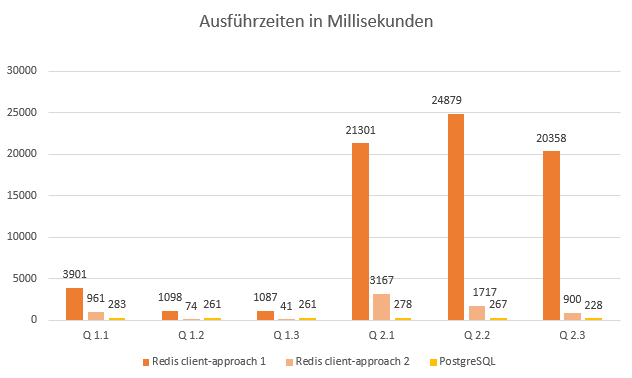
\includegraphics[width=1\textwidth]{pictures/results/results-client.png}
    \caption{Vergleich der Ausführzeiten in Millisekunden von Redis und PostgreSQL beim Client-Ansatz.}      % caption the image
    \label{pic:results-client}    % label the image for internal referencing
\end{figure}

Hinweis: Im Laufe der Forschung wurden verschiedene Varianten der Abfragen entwickelt, die sich hauptsächlich in Details unterscheiden. Für die Ergebnisse wurden hier jeweils die schnellsten Varianten ohne RediSearch-Aggregationen verwendet. Die genutzten Varianten haben folgende Bezeichnungen im Quellcode: \emph{Q1\_1\_client\_c}, \emph{Q1\_2\_client\_c}, \emph{Q1\_3\_client\_c}, \emph{Q2\_1\_client\_a}, \emph{Q2\_2\_client\_a}. Im Quellcode, der im digitalen Anhang zu finden ist, sind weitere Varianten enthalten.

% Noch was zu Q2.1

\subsubsection{Fazit}
% Warum nur bis Q2.2

\subsection{Ansatz 3: Serverseitige Joins}
\subsubsection{Aufbau der Daten}
Der Aufbau der Daten entspricht dem Aufbau der Daten im Client-Ansatz (siehe \cref{sec:client-approach-datastructure}). Dieser Ansatz unterscheidet sich lediglich in den Abfragen von dem anderen Ansatz.
\subsubsection{Aufbau der Abfragen}
\subsubsection{Ergebnisse}

% TODO: Position fixen
\begin{table}[h]
\centering
\begin{tabular}{lcc}
\hline
Query & Redis & PostgreSQL \\ \hline
Q 1.1 & 2545  & 283       \\
Q 1.2 & 98    & 261       \\ \hline
\end{tabular}
\caption{Vergleich der Ausführzeiten in Millisekunden von Redis und PostgreSQL beim Server-Ansatz.\\
 Die Messwerte wurden ermittelt, indem der Median von jeweils drei unmittelbar nacheinander durchgeführten Messungen gebildet wurde.}
\label{tab:results-server}
\end{table}

% TODO: Position fixen
\begin{figure}[ht]  % figure position
    \centering      % center the image
    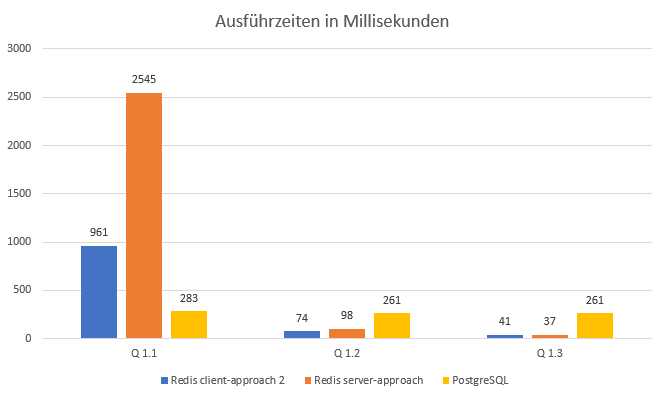
\includegraphics[width=1\textwidth]{pictures/results/results-server.png}
    \caption{Vergleich der Ausführzeiten in Millisekunden von Redis und PostgreSQL beim Server-Ansatz.}      % caption the image
    \label{pic:results-server}    % label the image for internal referencing
\end{figure}

Hinweis: Im Laufe der Forschung wurden verschiedene Varianten der Abfragen ent-
wickelt, die sich hauptsächlich in Details unterscheiden. Für die Ergebnisse wurden
hier jeweils die schnellsten Varianten verwendet. Die
genutzten Varianten haben folgende Bezeichnungen im Quellcode: \emph{Q1\_1\_server\_a}, \emph{Q1\_2\_server\_a}. Im Quellcode,
der im digitalen Anhang zu finden ist, sind weitere Varianten enthalten.


\subsubsection{Fazit}


\subsection{Ansatz 4: Denormalisiert}
\subsubsection{Aufbau der Daten}
\subsubsection{Aufbau der Abfragen}
\subsubsection{Ergebnisse}
\subsubsection{Fazit}